\documentclass{beamer}
\usefonttheme[onlymath]{serif}

\usepackage[utf8]{inputenc}
\usepackage[T1]{fontenc}
\usepackage{lmodern}
\usepackage[english]{babel}
%\frenchbsetup{CompactItemize=false}


% \usepackage[babel]{csquotes}
% \usepackage[url=false, doi=false, style=science, backend=bibtex, bibencoding=ascii]{biblatex}
% \bibliography{IEEEabrv,bib/OAM}

  
\graphicspath{{img/}}


\mode<presentation> {
	% \useoutertheme{infolines} % Pour les thèmes qui n'ont pas de pied-de-page
	\usetheme{ulaval}
	%\usecolortheme{ulaval}
	% \setbeamercovered{transparent}
	\setbeamercovered{invisible}
	%\setbeamertemplate{navigation symbols}{} % Enlever les icônes de navigation
}


%\usepackage{bm} 
% For typesetting bold math (not \mathbold)
%\includeonlyframes{}

%\usepackage{pgfpages}
%\setbeameroption{show notes on second screen}
%\setbeameroption{show notes}
%\setbeamertemplate{note page}[plain]

\logo{%\includegraphics[height=0.6cm]{COPL}\hspace{.5cm}%
	
\includegraphics[height=0.5cm]{UL_P}\hspace{.2cm}\vspace{.85\paperheight}}


\title[Utilisation de précurseurs textuels]{Utilisation de précurseurs textuels dans la gestion de risques extrèmes}
%\subtitle[]{}

\author[J-T Baillargeon]{Jean-Thomas Baillargeon}
\institute[Université Laval]
{
	École d'actuariat \\
	Université Laval, Québec, Canada \\
	\medskip
	{\emph{jean-thomas.baillargeon.1@ulaval.ca}}
}
\date{\today} % \today will show current date. 
% Alternatively, you can specify a date.


\AtBeginSection[]{
  \begin{frame}
	\Huge \centerline{\insertsection}
%  \small \tableofcontents[currentsection, hideothersubsections]
  \end{frame} 
}

\begin{document}



\begin{frame}[label=titre, plain]
	\titlepage
	\begin{center}%\includegraphics[height=1.2cm]{COPL}%
		%\hspace{2cm}
		
\includegraphics[height=2cm]{UL_P}\end{center}
\end{frame}



\begin{frame}[label=intro]{Introduction}
	\begin{itemize}
		\item Présentation de l'article de [trixier], Construction Safety Risk Modeling and Simulation.
		\item Survol de l'article de [trixier], Automated content analysis for construciton safety.	
		\item Articles tirés de la thèse doctorale [...]
	\end{itemize}
	\end{frame}


\begin{frame}[label=intro]{Mise en contexte}
	\begin{itemize}
		\item Secteur qui emploi 7\% de la population américaine.
		\item Secteur responsable de 17\% des morts au travail.
		\item Environ 700 morts par années.
		\item Il n'y pas que les décès! Secteur très risqué.
	\end{itemize}
	\end{frame}


\begin{frame}[label=intro]{État des choses}
	\begin{itemize}
		\item Évaluation des risques physiques (non monétaire.)
		\item Évaluation du niveau de risque d'une situation.
		\item Avis d'experts (avec biais cognitifs.)
		\item Données dans des rapport d'accidents	
	\end{itemize}
\end{frame}


\begin{frame}[label=intro]{Grand idée}
	\begin{itemize}
		\item Évaluer le niveau de risque d'une situation selon des mots clés.
		\item Évaluer le potentiel d'escalation d'une situation.
	\end{itemize}
\end{frame}


\begin{frame}[label=intro]{Agenda}
	\begin{itemize}
		\item Extraction des informations
		\begin{itemize}
			\item Natural Language Processing
			\item Lematisation, Part of speach tagging, Ngram 
			\item Pipeline d'entraînement et outils d'extraction
		\end{itemize}
		\item Évaluation du niveau de risque d'un situation
		\begin{itemize}
			\item Calcul du risque par mot clé
			\item Simulation pour obtenir une fonction de répartition
		\end{itemize}
		
		\item Évaluation du potentiel d'escalation d'une situation
			\begin{itemize}
				\item Modélisation du pire cas
				\item Simulation pour obtenir une copule 
			\end{itemize}
	\end{itemize}
\end{frame}









\section{Extraction des informations}

	\begin{frame}
		Que cherchons nous?\\
		Nous cherchons à découvrir les causes reliées aux accidents sur les chantiers de construction\\
		Qu'avaons nous à notre disposition?\\
		Nous avons les rapports d'accidents passés\\
	\end{frame}
\section{Analyse univariée}

\begin{frame}
	Prédiction et évaluation des risques
	\begin{itemize}
		\item Connaissances à transférer à la machine apprenante
		\begin{itemize}
			\item Prédire le risque relatif d'une sitation étant donnée certains précurseurs
		\end{itemize}	
		
		\item Éléments à modéliser
		\begin{itemize}
			\item fonction de densité des risques associés à la construction
		\end{itemize}	
	\end{itemize}
\end{frame}


\begin{frame}
	\begin{itemize}
	\item Données entrantes
	\begin{itemize}
		\item Banque de données de 921 rapport avec évaluation des sévérités par Esmaeili and Hallowell. Seuls 814 ont été conservés.
		\item La sévérité est sous-divisée en 5 classes.
		\item Extraction des précurseurs de risques de ces rapports avec l'outil développé plus tôt.
		\end{itemize}	
	\end{itemize}

	Valeur de la sévérité par type d'occurence
	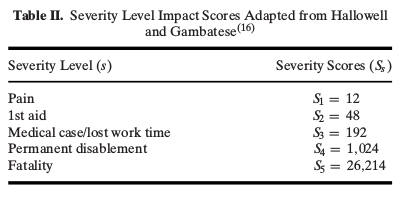
\includegraphics[width=300px]{table_severite}
\end{frame}

\begin{frame}
	On a maintenant la matrice creuse RP , \\
	\begin{tabular}[t]{lcccc}
		rapport & $w_1$ & $w_2$ & ... & $w_{80}$ \\
		$\textrm{rapport}_1$ & 1 & 0 &  & 1 \\
		$\textrm{rapport}_2$ & 1 & 0 &  & 1 \\
		$\textrm{rapport}_3$ & 0 & 1 &  & 1 \\
		... &  &  &  & \\
		$\textrm{rapport}_{814}$ & 1 & 1 &  & 1 \\
	\end{tabular}\\ 
	\bigskip
	et une table de vérité \\
	\begin{tabular}[t]{lc}
		rapport & sévérité  \\
		$\textrm{rapport}_1$ & $s_1$ \\
		$\textrm{rapport}_2$ & $s_2$ \\
		$\textrm{rapport}_3$ & $s_3$ \\
		... &  \\
		$\textrm{rapport}_{814}$ & $s_{814}$ \\
	\end{tabular}
\end{frame}

\begin{frame}
	Les auteurs ont fait une estimation de la valeur du risque $R_p$ pour chaque précurseur de la façon suivante\\
	$$R_p = \sum_{s=1}^{5} (n_{ps}S_s) $$
	avec $n_{ps}$ égal au nombre d'incident ayant une sévérité S le précurseur p est associé, et $S_s$ la valeur numérique du risque tel que vu à la Table II.\\
	\bigskip
	Les auteurs ont aussi corrigé les risques des précurseurs pour leur fréquece d'exposition.
	$$RR_p = \frac{1}{e_p} R_p$$
	avec $e_p$ la fréquence relative d'exposition d'un certain précurseur.
\end{frame}

\begin{frame}
	Petite note, l'article semble avoir une erreur concernant cette formule. Les codes R fournis par Trexier font une moyenne telle que 
	$$R_p = \frac{\sum_{s=1}^{5} (n_{ps}S_s)}{N}  $$
	avec $n_{ps}$ égal au nombre d'incident ayant une sévérité S le précurseur p est associé, $S_s$ la valeur numérique du risque tel que vu à la Table II, et N le nombre total de rapport analysés (N=814).\\
\end{frame}

\begin{frame}
	Maintenant que le risque par précurseur est déterminé, il est possible de recalculer le risque par rapport 
	$$R_{rapport_t} = \sum_{p=1}^{P} RR_p * \delta_{rp}$$
	avec $\delta_{rp}$ = 1 si le précurseur est présent dans le rapport et 0 autrement.
\end{frame}

\begin{frame}
	Autre petite note, faisons l'hypothèse que tous les précurseurs sont identiquement probable sur le chantier, de telle sorte que $e_p = 1, \forall p$ et ainsi que $RR_p = R_p$. \\
	\bigskip
	Il est ainsi possible de calculer l'erreur quadratique moyenne sur 
	$$\widehat{R_{rapport_t}} = \sum_{p=1}^{P} R_p * \delta_{rp}$$
	en comparant cette valeur avec $s_{rapport_t}$\\
	\bigskip
	Essaie de technique de régression en apprentissage automatique. Les modèles de séparateur a vaste marge (SVM), forêt aléatoire et régression linéaire seront comparées (train 85\%, test 15\%).
\end{frame}

\begin{frame}[c]
	Comparaison des erreur de régression 
	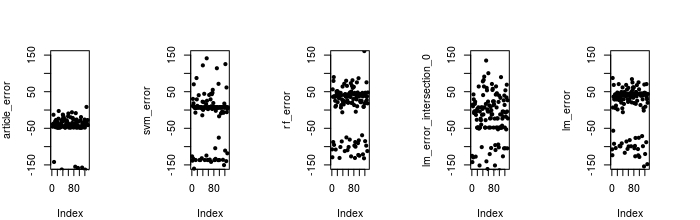
\includegraphics[width=330px] {error_comparison}
\end{frame}


\begin{frame}
	\textbf{Comparaison des erreur quadratiques moyennes}
	\begin{itemize}
		\item Méthode article: 1015
		\item SVM: 753
		\item Forêt aléatoires: 726
		\item Régression linéaire, intersection à 0: 794
		\item Régression linéaire: 710 
	\end{itemize}

	Il semble clairement y avoir un possibilité d'amélioration. Il faudrait réfléchir comment intégrer les poids des probabilité de trouver un précurseur sur le chantier. Est-ce qu'une nouvelle méthode de pondération (TFIDF / BNS) serait pertinente?
\end{frame}


\begin{frame}[t]
	Avec les $R_{rapport_t}$ calculés tel que dans l'article, \\
	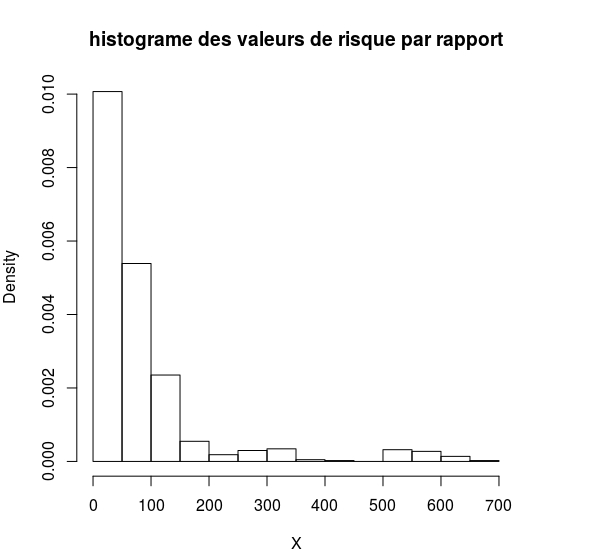
\includegraphics[height=200px] {histogramme_par_rapport}
	
\end{frame}


\begin{frame}[t]
	
	Modélisation de la fonction de densité
	\begin{itemize}
	\item Utilisation de noyaux pour estimer la densité (KDE) - pas EVT
\end{itemize}

Estimation par noyaux 

\begin{itemize}
	\item $\widehat{f(x)} = \frac{1}{nh} \sum^{n}_{i=1}K\big{(} \frac{x-x_i}{h},h \big{)}$
	\item choix d'un noyau N(0,1), avec fonction de densité $\frac{1}{\sqrt{2\pi}}e^{-x^2/2}$
	\item $\widehat{f(x)} = \frac{1}{n(2h^2\pi)^{p/2}}\sum^{n}_{i=1}e^{\frac{-1}{2}\big{(}\frac{x_{i}-x}{h}\big{)}^2}$
	\item choix de $h = \frac{0.9 \textrm{min}(\sigma^2, \frac{Q_3-Q_1}{1.34})}{n^{1/5}}$
\end{itemize}


Simulation pour enrichir la fonction de densité

\begin{itemize}
	\item Utilisation d'une méthode de bootstrap lissée
	\item Algorithme pour j simulation prenant R rapports en entrée:
		\begin{enumerate}		
		\item choisir un nombre entre 1 et R 
		\item tirer alétoirement $\epsilon_j$ avec $\epsilon_j \sim N(0,h_{x^2})$ 		
		\item créer une observation $X_{sim_j} = \bar{X} + \frac{X_i - \bar{X} + \epsilon_j}{\sqrt{1+h_{x^2}/\hat{\sigma}^2_X}} 	$
		\end{enumerate}
	
\end{itemize}

\end{frame}



\begin{frame}[t]
	Avec les $R_{rapport_t}$ et $\widehat{f(x)}$ calculés tel que dans l'article, \\
	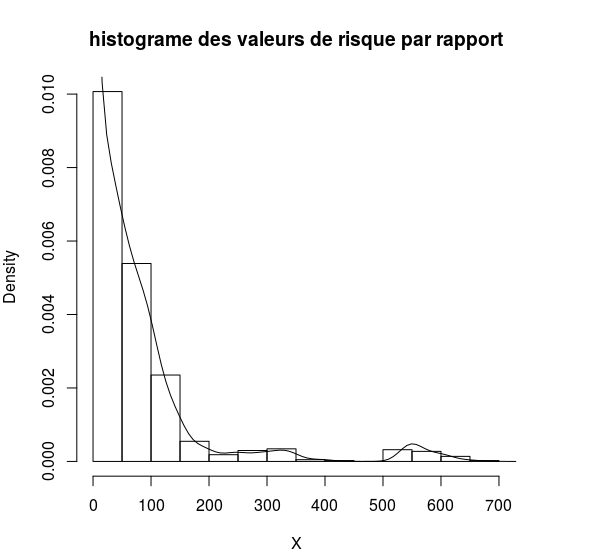
\includegraphics[height=200px] {histogramme_risque_rapport_kde}	
\end{frame}


\begin{frame}[t]
	Avec les $R_{rapport_t}$ et $\widehat{f(x)}$ calculés tel que dans l'article, \\
	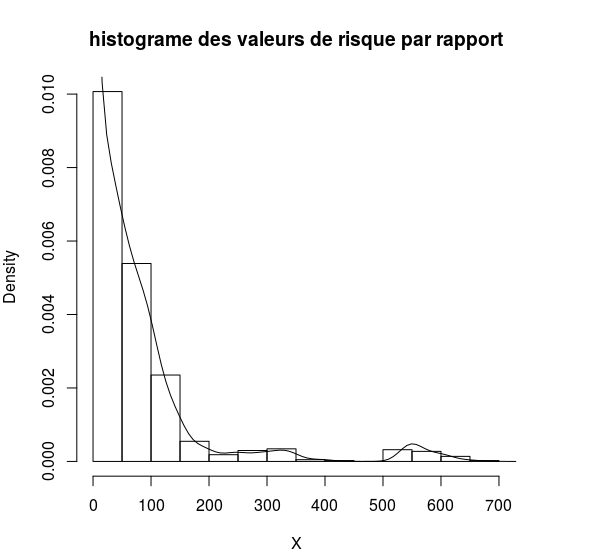
\includegraphics[height=200px] {histogramme_risque_rapport_kde}	
\end{frame}






\section*{Contents}

\begin{frame}[label=toc]{Outline}
	\setlength{\leftskip}{5cm}%
	\tableofcontents[subsectionstyle=show]
\end{frame}



\section{Main Section}

\subsection{List styles}

\subsubsection{Itemize}

\begin{frame}[label=itemize]\frametitle{Itemize sample} 
	\begin{itemize}
		\item Item 1
		\item Item 2
		\begin{itemize}
			\item Sub item 1
			\item Sub item 2
			\begin{itemize}
				\item Sub sub sub item 1
				\item Sub sub sub item 2
			\end{itemize}
			\item Sub item 3
		\end{itemize}
		\item Item 3
	\end{itemize}
\end{frame}

\subsubsection{Enumerate}

\begin{frame}[label=enumerate]\frametitle{Enumerate sample} 
	\begin{enumerate}
		\item Item 1
		\item Item 2
		\begin{enumerate}
			\item Sub item 1
			\item Sub item 2
			\begin{enumerate}
				\item Sub sub sub item 1
				\item Sub sub sub item 2
			\end{enumerate}
			\item Sub item 3
		\end{enumerate}
		\item Item 3
	\end{enumerate}
\end{frame}

\subsubsection{Description}

\begin{frame}[label=description]\frametitle{Description sample}
    
\begin{description}
	\item[Term 1:] Definition 1
	\item[Term 2:] Definition 2
	\item[Term 3:] Definition 3
\end{description}

\end{frame}

\subsection{Boxes styles}

\begin{frame}[label=boxes]\frametitle{Boxes Styles}
    
\begin{block}{Block Title}
	Block content
\end{block}

\begin{alertblock}{Alert Block Title}
	Alert block content
\end{alertblock}

\begin{exampleblock}{Example Block Title}
	Example block content
\end{exampleblock}

\end{frame}

\subsection{Block environments}

\begin{frame}[label=environments]\frametitle{Environments Samples}
    
	\begin{definition}
	Definition content
	\end{definition}
  
	\begin{example}
	Example content
	\end{example}

	\begin{proof}
	Proof content
	\end{proof}  
    
	\begin{theorem}
	Theorem content
	\end{theorem}

\end{frame}


\subsection{Math}

\begin{frame}[label=math]\frametitle{Math}
    
\begin{equation}
	V_0 = k_0 \rho \sqrt{n_1^2 - n_2^2}
\end{equation}

\end{frame}


\subsection{Text environments}

\begin{frame}[label=text]\frametitle{Text Environments}
    
\begin{quotation}
  Quotation environment line 1\\
  Quotation environment line 2
\end{quotation}
\begin{quote}
  Quote environment line 1\\
  Quote environment line 2
\end{quote}
\begin{semiverbatim}
  Semiverbatim environment
\end{semiverbatim}
\begin{verse}
  Verse environment line 1\\
  Verse environment line 2
\end{verse}  

\end{frame}

\section{Conclusion}

\begin{frame}[label=conclu]{Conclusion slide}
	That's all folks!
\end{frame}



% End of slides
\end{document}